\documentclass[border=4pt]{standalone}
\usepackage{amsmath,amssymb,tikz}
\usetikzlibrary{arrows.meta,calc,decorations.markings}
\begin{document}
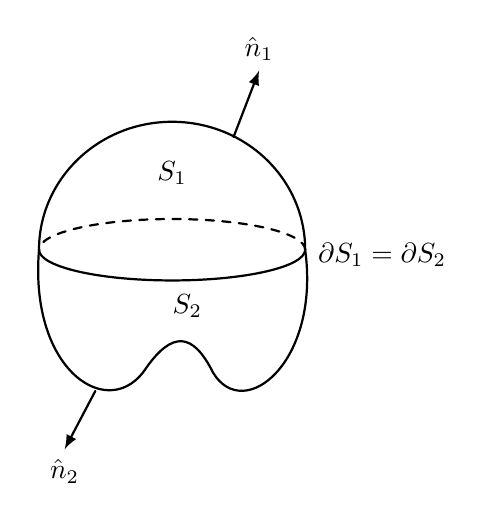
\begin{tikzpicture}[scale=1.3,>=latex,line cap=round]
  \draw[thick] (-1.3,0) arc (180:0:1.3 and 1.25);
  \draw[thick] (-1.3,0) .. controls (-1.4,-1.2) and (-0.6,-1.7) .. (-0.25,-1.15) .. controls (0,-0.8) and (0.2,-0.8) .. (0.4,-1.2) .. controls (0.7,-1.7) and (1.45,-1.1) .. (1.3,0);
  \draw[thick] (-1.3,0) arc (180:360:1.3 and 0.3);
  \draw[thick,dashed] (1.3,0) arc (0:180:1.3 and 0.3);
  
  \node at (0,0.75) {$S_1$};
  \node at (0.15,-0.55) {$S_2$};
  \draw[->,thick] (0.6,1.1) -- (0.85,1.75) node[above]{$\hat n_1$};
  \draw[->,thick] (-0.75,-1.38) -- (-1.05,-1.95) node[below]{$\hat n_2$};
  \node[right] at (1.33,-0.05) {$\partial S_1 = \partial S_2$};
\end{tikzpicture}
\end{document}
